%! Author = Runge
%! Date = 29-12-2023

% Preamble
\documentclass[runningheads]{llncs}
\overfullrule=10pt
\frenchspacing

% Packages
%! Author = Runge
%! Date = 29-12-2023

% Packages
\RequirePackage{setup/clrscode4e}
\usepackage{microtype}
\usepackage{mathtools, thm-restate}
\usepackage{stix2}
\usepackage{amsmath, amsthm}
\usepackage{booktabs}
\usepackage{tikz}

% Packages with options set
\usepackage[hidelinks]{hyperref}
\usepackage[textsize=small,obeyDraft]{todonotes}
\usepackage[newfloat, outputdir=../out]{minted}
\usepackage[backend=biber,
    bibencoding=utf8,
    maxbibnames=20,
    style=ieee,
    citestyle=numeric-comp,
    url=false
]{biblatex}
\usepackage[acronym]{glossaries}

% Hyperlink and PDF properties
\usepackage{orcidlink}
\makeatletter
\hypersetup{%
    plainpages=false,%
    pdftitle=\@title,%
    pdfauthor={Sebastian Aaholm, Lars Emanuel Hansen, Daniel Runge Petersen},%
    pdflang={en-GB},%
    pdfsubject={Semester project at Aalborg University},%
    pdfkeywords ={Formal Verification, Parameter Estimation, Decision Diagram}
    bookmarksnumbered=true,%
    colorlinks=true,%
    citecolor=black,%
    filecolor=black,%
    linkcolor=black,% you should probably change this to black before printing
    urlcolor=black,%
    pdfstartview=FitH%
}
\makeatother

% Package setup
\setlength{\marginparwidth}{2cm} % todonotes width
\setminted{linenos, autogobble, breaklines, fontsize=\footnotesize, style=friendly, xleftmargin=1em, numbersep=5pt}
\addbibresource{bib/main.bib}

% Other setup and options
\declaretheorem{theorem}
\declaretheorem{lemma}
\declaretheorem{corollary}
\declaretheorem{definition}
\declaretheorem{example}
\declaretheorem{conjecture}
\DeclareFloatingEnvironment[name=Algorithm, placement=htb!]{algorithm}

\makeglossaries

%! Author = Runge
%! Date = 29-12-2023

\newacronym{aau}{AAU}{Aalborg University}
\newacronym{mc}{MC}{Markov Chain}
\newacronym{hmm}{HMM}{Hidden Markov Model}
\newacronym{mdp}{MDP}{Markov Decision Process}
\newacronym{ctmc}{CTMC}{Continuous Time Markov Chain}
\newacronym{dtmc}{DTMC}{Discrete Time Markov Chain}
\newacronym{bw}{BW}{Baum-Welch}
\newacronym{add}{ADD}{Algebraic Decision Diagram}
\newacronym{bdd}{BDD}{Binary Decision Diagram}
\newacronym{pctmc}{pCTMC}{Parametric Continuous Time Markov Chain}
\newacronym{cudd}{CuDD}{Colorado University Decision Diagram}
\newacronym{cthmm}{CTHMM}{Continuous Time Hidden Markov Model}
\newacronym{iid}{i.i.d.}{independently identically distributed}
\newacronym{sul}{SUL}{System Under Learning}
\newacronym{nand}{NAND}{NAND multiplexing}
\newacronym{brp}{BRP}{Bounded Retransmission Protocol}

% % %! Author = Runge
% %! Date = 29-12-2023

\title{Baum-Welch Algorithm for Markov Models Using Algebraic Decision Diagrams}

%% For compsoc journal
\author{%
    Sebastian Aaholm\IEEEauthorrefmark{1},
    Lars Emanuel Hansen\IEEEauthorrefmark{2},
    Daniel Runge Petersen\orcidlink{0009-0004-6529-4342}\IEEEauthorrefmark{3},
    \IEEEcompsocitemizethanks{
        \IEEEcompsocthanksitem All authors are with the Dept. of Computer Science, Aalborg University, Aalborg, Denmark
        \IEEEcompsocthanksitem E-mails:
        \IEEEauthorrefmark{1}saahol20,
        \IEEEauthorrefmark{2}leha20,
        \IEEEauthorrefmark{3}dpet20\\ @student.aau.dk}
}


%! Author = Lars
%! Date = 10-03-2025

% \title{Baum-Welch Algorithm for Markov Models Using Algebraic Decision Diagrams}

% \author{Sebastian Aaholm\inst{1}
%     \and Lars Emanuel Hansen\inst{1}
%     \and Daniel Runge Petersen\inst{1}\orcidID{0009-0004-6529-4342}}

% \institute{Dept. of Computer Science, Aalborg University, Aalborg, Denmark}

% Document
\begin{document}
% %! Author = Runge
% %! Date = 29-12-2023

\title{Baum-Welch Algorithm for Markov Models Using Algebraic Decision Diagrams}

%% For compsoc journal
\author{%
    Sebastian Aaholm\IEEEauthorrefmark{1},
    Lars Emanuel Hansen\IEEEauthorrefmark{2},
    Daniel Runge Petersen\orcidlink{0009-0004-6529-4342}\IEEEauthorrefmark{3},
    \IEEEcompsocitemizethanks{
        \IEEEcompsocthanksitem All authors are with the Dept. of Computer Science, Aalborg University, Aalborg, Denmark
        \IEEEcompsocthanksitem E-mails:
        \IEEEauthorrefmark{1}saahol20,
        \IEEEauthorrefmark{2}leha20,
        \IEEEauthorrefmark{3}dpet20\\ @student.aau.dk}
}


%! Author = Lars
%! Date = 10-03-2025

% \title{Baum-Welch Algorithm for Markov Models Using Algebraic Decision Diagrams}

% \author{Sebastian Aaholm\inst{1}
%     \and Lars Emanuel Hansen\inst{1}
%     \and Daniel Runge Petersen\inst{1}\orcidID{0009-0004-6529-4342}}

% \institute{Dept. of Computer Science, Aalborg University, Aalborg, Denmark}
\maketitle
%! Author = Runge
%! Date = 29-12-2023

\begin{abstract}
    The \gls{bw} algorithm is a widely used method for training \glspl{hmm} and \glspl{mc} from observation sequences.
    However, traditional implementations using recursive or matrix-based methods often struggle with scalability due to redundancy and high memory consumption.
    This thesis proposes a novel, symbolic implementation of the \gls{bw} algorithm using \glspl{add}, which provide a compact and efficient representation of probabilistic models.
    We extend on \Cupaal, a C++ library that implements the \gls{bw} algorithm entirely with \glspl{add}, and integrate it into the \Jajapy\ library, resulting in a new symbolic learning tool referred to as \JajapyTwo.

    Our approach enables efficient learning from multiple observation sequences and supports both \glspl{hmm} and \glspl{mc}.
    Through experiments on models from the QComp benchmark set, we demonstrate that the symbolic implementation significantly improves performance for larger observation sets and models with repeated structures, while maintaining learning accuracy.
    These results affirm the potential of \gls{add}-based symbolic computation as a scalable alternative for probabilistic model learning.
\end{abstract}

\begin{IEEEkeywords}
    Algebraic Decision Diagrams, Baum-Welch Algorithm, Hidden Markov Models, Markov Chains, Model Checking
\end{IEEEkeywords}
%! Author = Runge
%! Date = 29-12-2023

\section{Introduction}\label{sec:introduction}
\IEEEPARstart{T}{he} Baum-Welch algorithm is a widely used method for training Markov models in applications such as speech recognition, bioinformatics, and financial modeling~\cite{chavan2013overview,ciocchetta2009bio,mamon2007hidden}.

Traditionally, the Baum-Welch algorithm relies on matrix-based or recursive approaches to estimate model parameters from observed sequences.

An example of this is the \Jajapy\ library~\cite{ReynouardIB23}, which implements the Baum-Welch algorithm using a recursive matrix-based approach.
This library is designed to learn probabilistic models from partially observable executions, producing observation sequences - also known as traces.

The key strength of \Jajapy\ lies in its flexibility to accommodate various learning scenarios, along with seamless integration into standard verification workflows using tools like \Storm\ and \Prism.
However, the performance of \Jajapy\'s Baum-Welch algorithm implementation has been a significant limitation, because of the inherent redundancy in matrix-based representations, which leads to inefficiencies particularly in terms of time and memory consumption, which restricts its scalability to larger models.

To address these challenges, we propose a novel approach that replaces conventional matrices and recursive formulations with \glspl{add}.
\glspl{add} provide a compact, structured representation of numerical functions over discrete variables, enabling efficient manipulation of large probabilistic models.

By leveraging \glspl{add}, we can exploit the sparsity and structural regularities of \glspl{hmm} and \glspl{mc}, significantly reducing memory consumption and accelerating computation.

This paper presents several contributions toward efficient learning of \glspl{hmm} and \glspl{mc} models, by leveraging \glspl{add}:

First, we extend the \gls{bw} algorithm for these models using symbolic computation, reformulating each algorithm step as operations on \glspl{add}, leveraging the CUDD library to carry out these operations symbolically using \glspl{add}.
This reformulation enables efficient calculation of the Markov models in a compact and scalable form.

Secondly, our approach extends previous work on symbolic calculation by accommodating learning from multiple observation sequences for both types of Markov models, broadening the applicability of symbolic learning.

Thirdly, we conduct an experimental evaluation of the scalability of the symbolic Baum-Welch algorithm for a \gls{mc} from the QComp benchmark set~\cite{HartmannsKPQR19}, which serves as a standard reference for evaluating the performance of probabilistic model checking algorithms.
Our findings suggest that replacing matrices and recursive formulations with \glspl{add} offers a scalable alternative, making Markov model-based learning feasible for larger and more complex datasets.

Additionally, we implement Python bindings for the \Cupaal\ tool, making it accessible and usable within Python-based machine learning and model-checking workflows, such as \Jajapy\footnote{Source code avaliable at: \url{https://github.com/AAU-Dat/CuPAAL}}.

Finally, using theses python bindings we integrate \Cupaal\ into \Jajapy\ as \JajapyTwo, enabling users to seamlessly run symbolic probabilistic learning algorithms within \Jajapy.

\section{Preliminaries}\label{sec:preliminaries}
This section provides an overview of the theoretical background necessary to understand the rest of the article.
We begin by defining the key concepts of a \gls{hmm} and a \gls{mc}, which are the two main models used in this report.


\subsection{Hidden Markov Model}\label{subsec:hmm}
\glspl{hmm} were introduced by Baum and Petrie in 1966~\cite{baum1966statistical} and have since been widely used in various fields, such as speech recognition~\cite{chavan2013overview}, bioinformatics~\cite{ciocchetta2009bio}, and finance~\cite{mamon2007hidden}.
\begin{definition}[Hidden Markov Model]
    A Hidden Markov Model (HMM) is a tuple $\mathcal{M} = (S, \mathcal{L}, \mathscr{l}, \tau,  \pi)$, where:
    \begin{itemize}
        \item $S$ is a finite set of states.
        \item $\mathcal{L}$ is a finite set of labels.
        \item $\mathscr{l}: S \rightarrow D(\mathcal{L})$ is the emission function.
        \item $\tau: S \rightarrow D(S)$ is the transition function.
        \item $\pi \in D(S)$ is the initial distribution.
    \end{itemize}
\end{definition}

$D(X)$ denotes the set of probability distributions over a  finite set $X$.
The emission function $\mathscr{l}$ describes the probability of emitting a label given a state.
The transition function $\tau$ describes the probability of transitioning from one state to another.
The initial distribution $\pi$ describes the probability of starting in a given state.
An \gls{hmm} is a statistical model that describes a system that evolves over time.
The system is assumed to hold the Markov property, meaning that the future state of the system only depends on the current state and not on the past states.
The system is also assumed to be unobservable, meaning that the states are hidden and cannot be directly observed.
Instead, the system emits observations, which are used to infer the hidden states.

An example of an \gls{hmm} is a weather model where the hidden state represents the actual weather (sunny, rainy, or cloudy), but we only observe indirect signals, such as whether someone is carrying an umbrella.

\subsection{Markov Chain}\label{subsec:mc}
A \gls{mc}, named after Andrei Markov, is a stochastic model widely used in different fields of study~\cite{Rabiner89}.
\begin{definition}[Markov Chain]
    A Markov Chain (MC) is a tuple $\mathcal{M} = (S, \mathcal{L}, \mathscr{l}, \tau,  \pi)$ identical to the HMM structure above except that the emission function is
    \emph{deterministic}: for every $s\in S$ there is a single label
    $l=\mathscr{l}(s)$ emitted with probability 1.
\end{definition}
In other words, the emission function $\mathscr{l}$ is a one-to-one mapping from states to labels.

A common example of an MC is a board game where a player moves between squares based on dice rolls.
Each square corresponds to a state, the dice rolls determine the transition probabilities, and the current square (state) is directly observable.

\subsection{Conversion between MCs and HMMs}\label{subsec:mc_hmm_conversion}
In this section, we will discuss the conversion between \glspl{mc} and \glspl{hmm}.
This conversion is important because it allows us to use the same algorithms and techniques for both models, even though they have different properties.
From the definition of a \gls{mc}, we can see that it is a special case of an \gls{hmm} where the emission function is deterministic.

\subsubsection{Markov Chains to Hidden Markov Models}\label{subsec:mc2hmm}
This conversion is straightforward because the components of the \gls{mc} and \gls{hmm} are the same.
\begin{definition}[Markov Chain to Hidden Markov Model]
    Given a \gls{hmm} $\mathcal{M} = (S, \mathcal{L}, \mathscr{l}, \tau,  \pi)$, we can convert it into a \gls{mc} $\mathcal{M}' = (S', \mathcal{L}', \mathscr{l}', \tau',  \pi')$ by defining the components as follows:
    \begin{itemize}
        \item $S' = S$.
        \item $\mathcal{L}' = \mathcal{L}$.
        \item $\mathscr{l}' =  \begin{cases}
                      1 & l=\mathscr{l}(s) \\
                      0 & \text{otherwise}
                  \end{cases}$
        \item $\tau' = \tau$.
        \item $\pi' = \pi$.
    \end{itemize}
\end{definition}
The \gls{mc} $\mathcal{M}'$ is equivalent to the \gls{hmm} $\mathcal{M}$, meaning that they have the same transition and emission probabilities.
The only difference is that the \gls{mc} has a trivial emission function, meaning that each state emits a single label with probability 1.

\subsubsection{Hidden Markov Models to Markov Chains}\label{subsec:hmm2mc}
Converting a \gls{hmm} to an equivalent \gls{mc} is more complex.
In a \gls{hmm}, the observations are probabilistically related to the states, which introduces ambiguity, as multiple states can emit the same observation.
To create a fully observable \gls{mc} that captures the behavior of a \gls{hmm}, we must encode both the hidden state and the emitted label into the state space.
\begin{definition}[Hidden Markov Model to Markov Chain]
    Conversely, let
    \(
    \mathcal{M}
    = (S, \mathcal{L}, \mathscr{l}, \tau, \pi)
    \)
    be a \gls{hmm}.
    We define the observable \gls{mc}
    \(
    \mathcal{M}'
    = (S', \mathcal{L}', \mathscr{l}', \tau', \pi')
    \)
    by:
    \begin{itemize}
        \item $S' = \{(s,l)\in S\times\mathcal{L}\}$%, the new state space encodes both hidden states and their possible emitted labels,
        \item $\mathcal{L}' = \mathcal{L}$%, the label space remains unchanged,
        \item $\mathscr{l}'(s,l) = l$%, each new state deterministically emits its label,
        \item $\tau'\big((s,l),(s',l')\big) = \tau(s,s')\;\mathscr{l}(s')(l')$%, the transition function is modified to account for the emission probabilities,
        \item $\pi'(s,l) = \pi(s)\;\mathscr{l}(s)(l)$%, the initial distribution is modified to account for the emission probabilities.
    \end{itemize}
    \textbf{Remark.}
    Here each ' symbol refers to an object of the \emph{derived MC}.  In
    particular, $\tau'$ is \emph{not} the original HMM transition; it acts on the
    expanded state space $S'$ and already incorporates the emission probability for
    the label $l'$.

    The mapping increases the state space size from $|S|$ to at most
    $|S|\cdot|\mathcal{L}|$, but yields a fully observable system amenable to
    standard MC analysis.
\end{definition}

The conversion between \glspl{mc} and \glspl{hmm} is important because it allows us to use the same algorithms and techniques for both models, even though they have different properties.

\section{Methodology}\label{sec:methodology}
This is a section.

\subsection{Decision Diagrams}\label{subsec:decision-diagrams}
\acrfullpl{bdd} are data structures for efficiently representing and manipulating Boolean functions.
They are a compressed representation of truth tables, capturing the logical structure of a function in a graph-based format by eliminating redundancy, reducing memory usage, and improving computational efficiency~\cite{bryant1986graph}.

A \gls{bdd} is a directed acyclic graph derived from a decision tree, where each non-terminal node represents a Boolean variable, edges correspond to binary assignments (0 or 1), and terminal nodes store function values (0 or 1).
To reduce the size of the decision tree, \glspl{bdd} exploit redundancy by merging equivalent substructures, resulting in a canonical form (when reduced and ordered) that allows for efficient operations such as function evaluation, equivalence checking, and Boolean operations~\cite{bryant1986graph}.

\glspl{bdd} have been widely used in formal verification, model checking, and logic synthesis due to their ability to compactly represent large Boolean functions while maintaining efficient computational properties.
However, \glspl{bdd} suffer from exponential blowup in certain cases, particularly when dealing with functions that lack inherent structure or when representing numerical computations that go beyond Boolean logic.

\subsubsection{From BDDs to ADDs}\label{subsubsec:adds}
\acrfullpl{add} generalize the concept of \glspl{bdd} by allowing terminal nodes to take values beyond Boolean constants (0 and 1).
Instead of restricting values to true/false, \glspl{add} can store arbitrary numerical values, making them useful for representing and manipulating functions over discrete domains~\cite{bahar1997algebric}.
This generalization enables the efficient representation of functions such as cost functions~\cite{kwiatkowska2004probabilistic}, probabilities~\cite{baier1997symbolic}, and other numerical relationships that arise in probabilistic reasoning.

The fundamental structure of an \gls{add} remains similar to a \gls{bdd}, where a decision tree is compacted by merging redundant substructures.
However, instead of performing Boolean operations, \glspl{add} allow for arithmetic operations such as addition and multiplication, making them well-suited for applications like dynamic programming, \glspl{mdp}, and linear algebraic computations~\cite{bahar1997algebric}.

\subsection{Recursive vs. Matrix vs. ADD-based Approaches}\label{subsec:approaches}
When designing algorithms for solving complex problems, different approaches can be taken to optimize computational efficiency.
Three common strategies are recursive, matrix-based, and \gls{add}-based approaches, each with distinct advantages and limitations.
\begin{itemize}
    \item \textbf{Recursive Approach:} Conceptually simple, recursion follows a divide-and-conquer strategy but can suffer from exponential time complexity due to redundant computations of overlapping subproblems~\cite[Chapter 4]{cormen2022introduction}.
    \item \textbf{Matrix Representation:} Reformulating algorithms using matrix operations leverages algebraic properties for parallel computation and efficient processing.
          However, matrix-based methods can be memory-intensive, particularly for sparse or structured data~\cite[Chapter 4, 15 \& 28]{cormen2022introduction}.
    \item \textbf{ADD-based Approach:} \glspl{add} provide a compact representation that eliminates redundancy in recursive computations.
          By reusing previously computed substructures, they improve efficiency and reduce memory overhead~\cite{bahar1997algebric}.
          Compared to matrices, \glspl{add} can offer a more space-efficient alternative for structured data while extending \gls{bdd} techniques to handle both Boolean and numerical computations.
\end{itemize}

In this work we explore the benefits of \gls{add}-based approaches for solving complex problems, focusing on parameter estimation in \glspl{dtmc} and \glspl{ctmc}.
We compare the performance of \gls{add}-based algorithms against recursive-based implementations, highlighting the advantages of using \glspl{add} for efficient computation and memory management.

\section{Experiments}\label{sec:experiments}
In this section, we describe the experiments conducted to evaluate the performance of the symbolic implementation of the Baum-Welch algorithm in the CuPAAL library by comparing it to the recursive implementation in Jajapy.
The evaluation is based on two key aspects: execution time and accuracy.

We conduct two experiments:
\begin{itemize}
    \item \textbf{Performance Comparison} - Measuring runtime and accuracy across different models.
    \item \textbf{Scalability Analysis} - Evaluating performance as the number of states increases.
\end{itemize}

Through these experiments, we aim to answer the following research questions:
\begin{itemize}
    \item \textbf{Question 1}: How does the symbolic implementation of the Baum-Welch algorithm in CuPAAL compare to the recursive implementation in Jajapy in terms of runtime and accuracy?
    \item \textbf{Question 2}: How does the performance of the CuPAAL implementation scale with the size of the model?
\end{itemize}

\subsection{Experimental Setup}
All experiments are conducted using a set of \glspl{dtmc} and \glspl{ctmc} obtained from publicly available benchmarks~\cite{hartmanns2019quantitative}
\footnote{The models are available at \url{https://qcomp.org/benchmarks/}. The models are Leader\_sync, Brp, Crowds, Mapk, Cluster, and Embedded.}~\cite{hartmanns2019quantitative}.

Each experiment is run ten times.
We report the average runtime (full run and per iteration), the average number of iterations, log-likelihood per iteration, and the type of error based on the model type.

Experiments stop when reaching a convergence threshold of 0.05 (the Jajapy default) or a 4-hour runtime limit. The final iteration's results are recorded.

The training data is randomly generated based on these models, consisting of 30 observation sequences of length 10 for each model.

The implementations used are:
\begin{enumerate}
    \item The original Jajapy implementation.
    \item The symbolic CuPAAL implementation.
\end{enumerate}

\subsection{Experiment 1: Performance Comparison of Implementations}
The first experiment is based on the ideas from the experiment conducted in~\cite{reynouard2024learning}.

We split this experiment into two separate analyses: one focusing on \glspl{dtmc} and another on \glspl{ctmc}. Since \glspl{dtmc} estimate probabilities while \glspl{ctmc} estimate rates, we use different error measures for accuracy evaluation.

The experiments evaluate the efficiency and accuracy of the symbolic approach (CuPAAL) versus the recursive approach (Jajapy). We measure:
\begin{itemize}
    \item \textbf{Runtime Efficiency} - The average time per run.
    \item \textbf{Convergence Speed} - The average number of iterations required.
    \item \textbf{Accuracy} - Measured using log-likelihood and an average error.
\end{itemize}

\textbf{Log-likelihood:} Measures how well a learned model explains observed data.
For a given observation sequence $O$ and model $M$, it is defined as:
\begin{equation}
    \begin{aligned}
        \log P(O \mid M) = \sum_{t=1}^{T} \log P(O_t \mid M)
    \end{aligned}
\end{equation}
where $P(O_t|M)$ is the probability of observing $O_t$ given the model.

\subsubsection{Experiment 1A: Accuracy Comparison for DTMCs}
For \glspl{dtmc}, the models used are shown in \autoref{tab:dtmc_models}.
For \glspl{dtmc}, we use the absolute error as the measure of accuracy, because in \glspl{dtmc} we are estimating probabilities, and we are interested in the absolute difference between the real value and the estimated value.

The absolute error is calculated as follows:
\begin{equation}
    \begin{aligned}
        \text{Absolute Error} = |r - e|
    \end{aligned}
\end{equation}
where $r$ is the real value and $e$ is the expected value.

\subsubsection{Experiment 1B: Accuracy Comparison for CTMCs}
For \glspl{ctmc}, the models used are shown in \autoref{tab:ctmc_models}.

For \glspl{ctmc}, we use relative error as the measure of accuracy, since rates in CTMCs can vary significantly in magnitude, an absolute difference may not properly reflect the accuracy.
For example, a difference of 0.1 in a transition rate of 0.2 is a large error, whereas the same difference in a rate of 10 is negligible.
Using relative error ensures that errors are proportional to the expected value.

The relative error is calculated as follows:
\begin{equation}
    \begin{aligned}
        \text{Relative Error} = \cfrac{|r - e|}{e}
    \end{aligned}
\end{equation}
where $r$ is the real value and $e$ is the expected value.

\begin{table}[!htb]
    \centering
    \caption{DTMC models}
    \label{tab:dtmc_models}
    \begin{tabular}{ll}
        \toprule
        Name         & Number of States \\
        \midrule
        Leader\_sync & 274              \\
        %Oscillators  & 453              \\
        Brp          & 886              \\
        Crowds       & 1145             \\
        \bottomrule
    \end{tabular}
\end{table}

\begin{table}[!htb]
    \centering
    \caption{CTMC models}
    \label{tab:ctmc_models}
    \begin{tabular}{lll}
        \toprule
        Name     & Number of States \\
        \midrule
        Mapk     & 118              \\
        Cluster  & 820              \\
        Embedded & 3480             \\
        \bottomrule
    \end{tabular}
\end{table}


\subsection{Scalability Experiment}
The primary objective of this experiment is to evaluate the scalability of the proposed symbolic implementation of the Baum-Welch algorithm in comparison to the recursive implementation in Jajapy.
Specifically, we aim to measure the time required to learn \glspl{dtmc} and \glspl{ctmc} over the number of states.
We measure:
\begin{itemize}
    \item \textbf{Runtime efficiency} - The average time per run.
\end{itemize}

For this experiment, we selected two models-\textit{leader\_sync} (\gls{dtmc}) and \textit{polling} (\gls{ctmc})—as they represent those used in the performance comparison experiment and scale well to large state spaces.

\subsubsection{Experiment 2A: Scalability for DTMCs}
In this experiment, we evaluate the scalability of CuPAAL for \glspl{dtmc} by measuring runtime efficiency as the number of states increases.
We use the \textit{leader\_sync} model, scaling from 26 to 1050 states.

This experiment provides insights into how the symbolic approach scales as model complexity increases.

\subsubsection{Experiment 2B: Scalability for CTMCs}
In this experiment, we evaluate the scalability of CuPAAL for \glspl{ctmc} by measuring runtime efficiency as the number of states increases.
We use the \textit{polling} model, scaling from 36 to 1334 states.

This experiment provides insights into how the symbolic approach scales as model complexity increases.

\section{Improvements}\label{sec:improvements}
This section outlines the improvements gained by transitioning from the recursive implementation in Jajapy to the symbolic approach in CuPAAL.

As discussed in (Ref to previous section talking about Jajapy), Jajapy uses a recursive implementation of the Baum-Welch algorithm to learn \glspl{hmm}.
In contrast, CuPAAL implements the Baum-Welch algorithm using \glspl{add}.
By leveraging \glspl{add}, CuPAAL demonstrates significant improvements over the recursive approach used in Jajapy.
The discussion of these improvements is based on the experimental results presented in Section~\ref{sec:experiments}.

\subsection{Run Time}\label{subsec:improvements_run_time}
One of the most notable advantages of CuPAAL over Jajapy is the reduction in run time, particularly for models with a large number of states.

The use of \glspl{add} minimizes redundant computations by merging identical values within the structure.
This optimization significantly reduces the computational needs, compared to a recursive implementation.
As a result, the run time gap between CuPAAL and Jajapy increases as the number of states grows, making CuPAAL a more scalable solution for large \glspl{hmm}.

The number of iterations of CuPAAL for each model is also slightly reduced compared to Jajapy.

This advantage is particularly beneficial in scenarios where handling large probability matrices would otherwise lead to excessive computational costs.


\subsection{Accuracy}\label{subsec:improvements_accuracy}
While run time is a key advantage of CuPAAL, it is equally important to assess whether these performance gains come at the cost of accuracy.
Since both approaches implement the Baum-Welch algorithm, they are expected to converge to similar model parameters when learning \glspl{hmm}.

As shown in Section~\ref{sec:experiments}, CuPAAL achieves accuracy comparable to Jajapy across various models.
These results can be seen in the values of avg delta and the log-likelihood, where the closer the value is to 0 the better.
Displaying that a symbolic implementation does not introduce significant numerical errors, ensuring that the learned transition and emission probabilities remain consistent with those obtained using the recursive approach.

Furthermore, by eliminating redundant calculations, CuPAAL may reduce floating-point errors that typically accumulate in recursive implementations.
Importantly, CuPAAL maintains accuracy even as the number of states increases, showcasing that its efficiency improvements do not compromise learning quality.
This makes it particularly well-suited for handling large-scale \glspl{hmm}.


\subsection{Implementation}\label{subsec:improvements_implementation}
The implementation of CuPAAL has been done in c++, compared to Jajapy which is implemented in Python.
This could also be a factor aiding the performance improvement of CuPAAL, as C++ is generally faster at computation compared to Python.
This choice of implementation not only improves speed but also ensures that CuPAAL can efficiently handle large models that would be infeasible in Python.

\subsection{Final improvement overview}\label{improvements_overview}
The improvements introduced by CuPAAL stem from multiple factors: the adoption of \glspl{add}, optimized run time and a high-performance C++ implementation.
These enhancements make CuPAAL a powerful alternative to recursive approaches like Jajapy, particularly when working with large, redundant, and complex \glspl{hmm}.






\section{Previous Work}\label{sec:jajapy_and_cupaal}
In this section, we provide a brief overview of previous work that has influenced our research and has been iterated upon.
Specifically, we discuss what these tools are, how they function, who utilizes them, and the motivations behind integrating them into our research.
The focus will be on two primary tools: Jajapy and CuPAAL.


\subsection{Jajapy}\label{sec:jajapy}
\Jajapy\ provides learning algorithms designed to construct accurate models of a system under learning (SUL) from observed traces.
Once learned, these models can be directly exported for formal analysis in tools such as \Storm~and \Prism.

\begin{figure}[!htb]
    \centering
    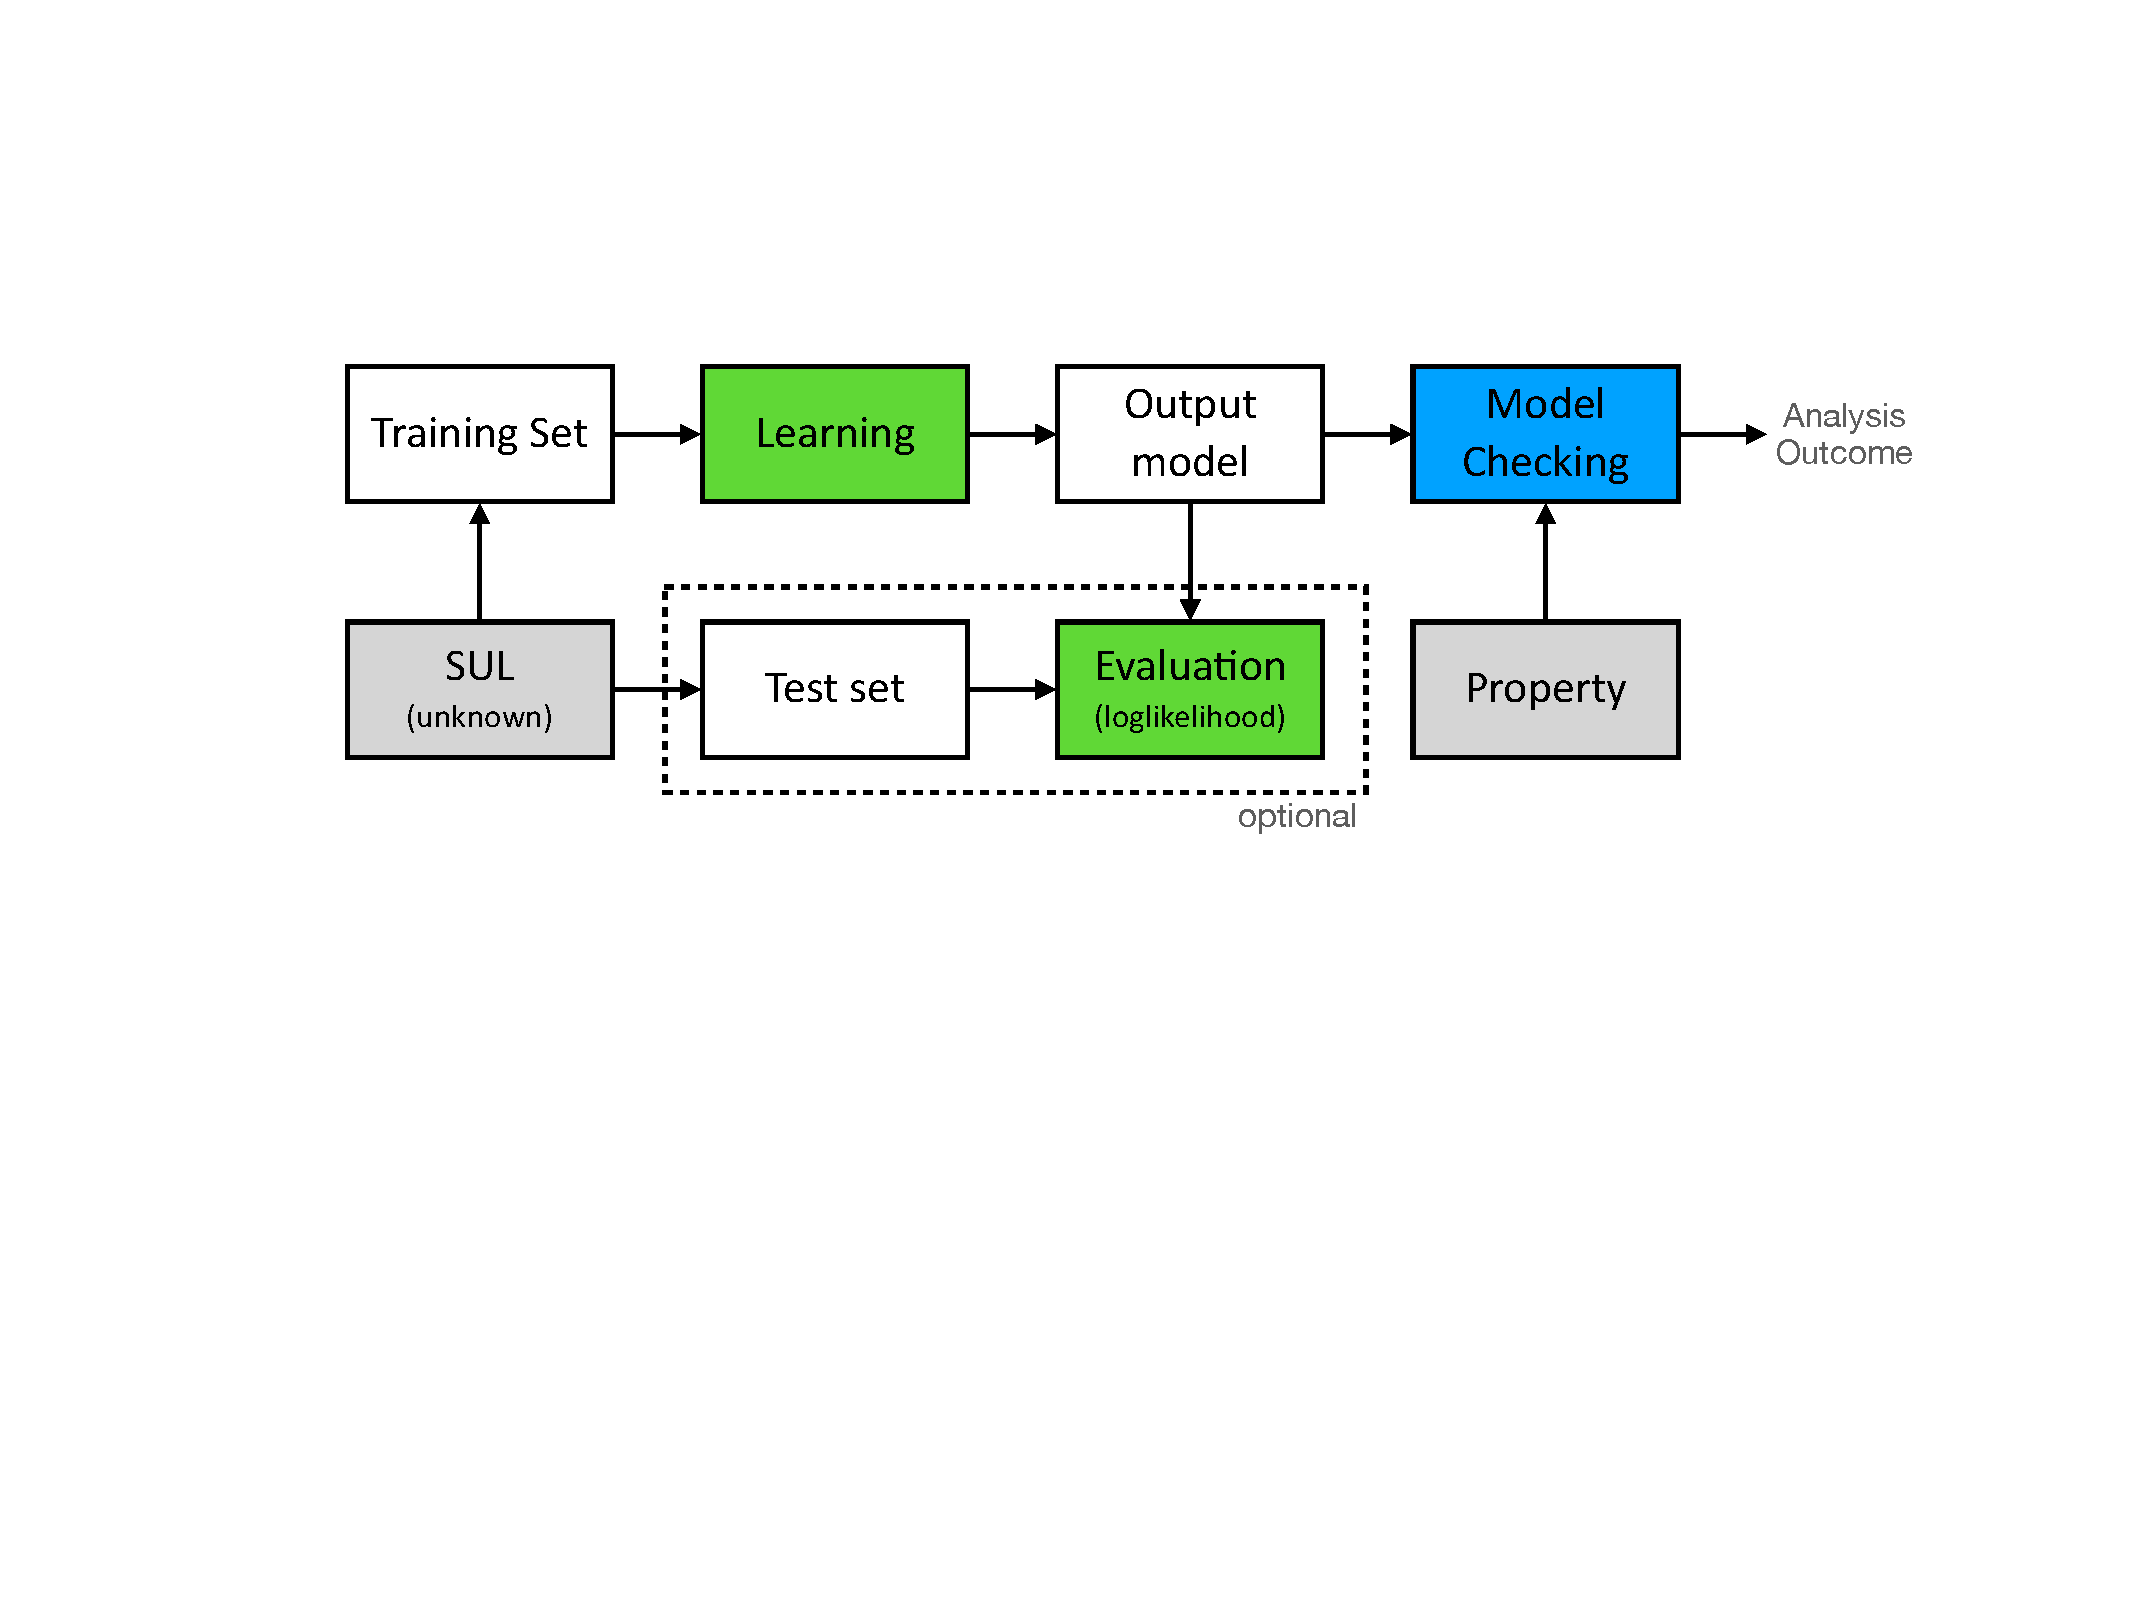
\includegraphics[width=0.9\textwidth]{figures/workflow.pdf}
    \caption{Modeling and verification workflow using \Jajapy. Phases involving \Jajapy\ are highlighted in green, while the blue phase represents verification using \Storm~or \Prism.}
    \label{fig:workflow}
\end{figure}

In this context, we refer to the \textit{training set} as the collection of observation traces used to infer a model of the SUL, and the \textit{test set} as a separate set of traces used to evaluate the quality of the learned model.

\Jajapy\ supports learning various types of models, depending on the structure of the training data.
For clarity, this paper focuses specifically on the new features introduced in \JajapyTwo, which primarily target Markov chains.
However, these improvements are equally applicable to other classes of Markov models supported by the tool.

At the core of \Jajapy's learning capabilities are several variants of the Baum-Welch (BW) algorithm~\cite{Baum70,Rabiner89}, adapted for discrete-time Markov chains (MCs), Markov decision processes (MDPs)\cite{BacciILR21}, and continuous-time Markov chains (CTMCs)\cite{BacciILR23}.
Each algorithm requires two inputs: a training set and the desired number of states for the output model.
The process begins with the creation of a randomly initialized model (e.g., a Markov chain) and iteratively updates its transition probabilities, increasing the likelihood of transitions that better explain the observed traces.

The efficiency and accuracy of the learning process depend heavily on the choice of the initial hypothesis.
To improve convergence and model quality, \Jajapy\ allows users to supply a custom initial hypotheses in several formats, including \Stormpy~sparse models, \Prism~files, or native \Jajapy\ model definitions.

An example of using \Jajapy\ to learn a 10-state Markov chain from a training set, starting from a random initial hypothesis, is shown in \autoref{fig:run-bw}.

\begin{listing}
    \begin{minted}{python} 
    from jajapy import BW 
    type(training_set) # list 
    output_model = BW().fit(training_set, nb_states=10) type(output_model) # stormpy.SparseDtmc 
    \end{minted}
    \caption{Example of using \Jajapy's BW implementation to learn a 10-state Markov chain from a training set.}
    \label{fig:run-bw}
\end{listing}

%Beyond the Baum-Welch algorithm, \Jajapy\ also includes implementations of Alergia~\cite{CarrascoO94,CarrascoO99} and IOAlergia~\cite{Mao11,MaoCJNLN16}, which are alternative algorithms for learning MCs and MDPs, respectively.
%These approaches require both a training set and a user-defined \textit{confidence} parameter.

Once a model has been learned, \Jajapy\ supports direct verification of properties using \Storm, provided the properties are supported.
Alternatively, the model can be exported to \Prism's format for verification using the \Prism\ model checker.


\subsection{CuPAAL}\label{subsec:cupaal}
CuPAAL is a tool developed in C++ that extends the work done in Jajapy by implementing the Baum-Welch algorithm with an \gls{add}-based approach instead of a recursive method.
The goal of CuPAAL is to leverage \glspl{add} to improve the efficiency of learning Markov models, particularly in large-scale applications where traditional recursive methods may become computationally expensive.

CuPAAL has undergone multiple iterations. Initially, it implemented a partial \gls{add}-based approach, where only certain components of the Baum-Welch algorithm were optimized using \glspl{add}.
This partial implementation served as an initial proof-of-concept to determine whether incorporating \glspl{add} could yield performance benefits compared to the recursive approach employed by Jajapy.

Following promising results from the partial implementation, further development led to a fully \gls{add}-based version of CuPAAL.
This iteration replaced all recursive computations with \glspl{add}, enabling more efficient execution, particularly for large models.
The transition to a fully \gls{add}-based approach demonstrated the potential for significant computational savings and scalability improvements, reinforcing the viability of this method for broader applications beyond our initial research scope.

By building upon Jajapy and developing CuPAAL, we have been able to evaluate the impact of using \glspl{add} in probabilistic model learning.




\printglossary[type=\acronymtype]

\printbibliography

\appendix % You can use \appendix if you only have a single appendix
\section{Cheatsheet}\label{sec:cheatsheet}
% If something is represented with a greek letter, it is something we calculate.

\begin{table}[htb!]
    \centering
    \caption{Symbol table.}
    \begin{tabular}{ll}
        \toprule
        \textbf{Symbol}                 & \textbf{Meaning}                                \\
        \midrule
        $\mathbb{R}$                    & Real numbers                                    \\
        $\mathbb{B}$                    & Boolean domain                                  \\
        $\mathbb{N}$                    & Natural numbers                                 \\
        $\mathcal{M}$                   & Markov Model                                    \\
        $s \in S$                       & States                                          \\
        $l \in L$                       & Labels                                          \\
        $o \in O \in \mathcal{O}$       & Observations                                    \\
        $t \in T$                       & Time steps                                      \\
        $\mathbf{1}$                    & Column vector of ones                           \\
        $\pi$                           & Initial distribution                            \\
        $\tau$                          & Transition function                             \\
        $\omega$                        & Emission function                               \\
        $\alpha$                        & Forward probabilities                           \\
        $\beta$                         & Backward probabilities                          \\
        $\gamma$                        & State probabilities given O                     \\
        $\xi$                           & Transition probabilities given O                \\
        $\lambda = (\pi, \tau, \omega)$ & Model Parameters                                \\
        %$\phi$ or $\psi$                & Scheduler                                       \\
        $\mu$                           & Mean                                            \\
        $\sigma$                        & Standard deviation                              \\
        $\theta = (\mu, \sigma^2)$      & Parameters of a distribution                    \\
        $P(\mathcal{O}; \lambda)$       & Probability of $\mathcal{O}$ given $\lambda$    \\
        $\ell(\lambda ;\mathcal{O})$    & Log likelihood of $\lambda$ under $\mathcal{O}$ \\
        $\cdot$                         & Scalar product                                  \\
        $\odot$                         & Hadamard product                                \\
        $\otimes$                       & Kronecker product                               \\
        $\oslash$                       & Hadamard division                               \\
        $\smblkcircle$                  & Transposed Khatri-Rao product                   \\
        \bottomrule
    \end{tabular}
    \label{tab:symbol-table}
\end{table}


\end{document}
